% Options for packages loaded elsewhere
\PassOptionsToPackage{unicode}{hyperref}
\PassOptionsToPackage{hyphens}{url}
\PassOptionsToPackage{dvipsnames,svgnames,x11names}{xcolor}
%
\documentclass[
  12pt,
]{article}
\author{}
\date{\vspace{-2.5em}}

\usepackage{amsmath,amssymb}
\usepackage{lmodern}
\usepackage{iftex}
\ifPDFTeX
  \usepackage[T1]{fontenc}
  \usepackage[utf8]{inputenc}
  \usepackage{textcomp} % provide euro and other symbols
\else % if luatex or xetex
  \usepackage{unicode-math}
  \defaultfontfeatures{Scale=MatchLowercase}
  \defaultfontfeatures[\rmfamily]{Ligatures=TeX,Scale=1}
  \setmainfont[]{Palatino}
\fi
% Use upquote if available, for straight quotes in verbatim environments
\IfFileExists{upquote.sty}{\usepackage{upquote}}{}
\IfFileExists{microtype.sty}{% use microtype if available
  \usepackage[]{microtype}
  \UseMicrotypeSet[protrusion]{basicmath} % disable protrusion for tt fonts
}{}
\makeatletter
\@ifundefined{KOMAClassName}{% if non-KOMA class
  \IfFileExists{parskip.sty}{%
    \usepackage{parskip}
  }{% else
    \setlength{\parindent}{0pt}
    \setlength{\parskip}{6pt plus 2pt minus 1pt}}
}{% if KOMA class
  \KOMAoptions{parskip=half}}
\makeatother
\usepackage{xcolor}
\IfFileExists{xurl.sty}{\usepackage{xurl}}{} % add URL line breaks if available
\IfFileExists{bookmark.sty}{\usepackage{bookmark}}{\usepackage{hyperref}}
\hypersetup{
  colorlinks=true,
  linkcolor={teal},
  filecolor={Maroon},
  citecolor={teal},
  urlcolor={teal},
  pdfcreator={LaTeX via pandoc}}
\urlstyle{same} % disable monospaced font for URLs
\usepackage[left=3cm,right=3cm,top=2cm,bottom=2cm]{geometry}
\usepackage{longtable,booktabs,array}
\usepackage{calc} % for calculating minipage widths
% Correct order of tables after \paragraph or \subparagraph
\usepackage{etoolbox}
\makeatletter
\patchcmd\longtable{\par}{\if@noskipsec\mbox{}\fi\par}{}{}
\makeatother
% Allow footnotes in longtable head/foot
\IfFileExists{footnotehyper.sty}{\usepackage{footnotehyper}}{\usepackage{footnote}}
\makesavenoteenv{longtable}
\usepackage{graphicx}
\makeatletter
\def\maxwidth{\ifdim\Gin@nat@width>\linewidth\linewidth\else\Gin@nat@width\fi}
\def\maxheight{\ifdim\Gin@nat@height>\textheight\textheight\else\Gin@nat@height\fi}
\makeatother
% Scale images if necessary, so that they will not overflow the page
% margins by default, and it is still possible to overwrite the defaults
% using explicit options in \includegraphics[width, height, ...]{}
\setkeys{Gin}{width=\maxwidth,height=\maxheight,keepaspectratio}
% Set default figure placement to htbp
\makeatletter
\def\fps@figure{htbp}
\makeatother
\setlength{\emergencystretch}{3em} % prevent overfull lines
\providecommand{\tightlist}{%
  \setlength{\itemsep}{0pt}\setlength{\parskip}{0pt}}
\setcounter{secnumdepth}{-\maxdimen} % remove section numbering
\newlength{\cslhangindent}
\setlength{\cslhangindent}{1.5em}
\newlength{\csllabelwidth}
\setlength{\csllabelwidth}{3em}
\newlength{\cslentryspacingunit} % times entry-spacing
\setlength{\cslentryspacingunit}{\parskip}
\newenvironment{CSLReferences}[2] % #1 hanging-ident, #2 entry spacing
 {% don't indent paragraphs
  \setlength{\parindent}{0pt}
  % turn on hanging indent if param 1 is 1
  \ifodd #1
  \let\oldpar\par
  \def\par{\hangindent=\cslhangindent\oldpar}
  \fi
  % set entry spacing
  \setlength{\parskip}{#2\cslentryspacingunit}
 }%
 {}
\usepackage{calc}
\newcommand{\CSLBlock}[1]{#1\hfill\break}
\newcommand{\CSLLeftMargin}[1]{\parbox[t]{\csllabelwidth}{#1}}
\newcommand{\CSLRightInline}[1]{\parbox[t]{\linewidth - \csllabelwidth}{#1}\break}
\newcommand{\CSLIndent}[1]{\hspace{\cslhangindent}#1}
\usepackage[labelsep=period]{caption}
\usepackage[labelfont=bf]{caption}
\usepackage[switch]{lineno}
\usepackage{type1cm} % scalable fonts
\usepackage{lettrine}
\usepackage{booktabs}
\usepackage{sectsty} \sectionfont{\centering}
\usepackage{caption}
\captionsetup[figure]{font=footnotesize}
\captionsetup[table]{font=footnotesize}
\captionsetup[table]{justification=centerlast}
\captionsetup[figure]{justification=centerlast}
\usepackage{booktabs}
\usepackage{longtable}
\usepackage{array}
\usepackage{multirow}
\usepackage{wrapfig}
\usepackage{float}
\usepackage{colortbl}
\usepackage{pdflscape}
\usepackage{tabu}
\usepackage{threeparttable}
\usepackage{threeparttablex}
\usepackage[normalem]{ulem}
\usepackage{makecell}
\usepackage{xcolor}
\ifLuaTeX
  \usepackage{selnolig}  % disable illegal ligatures
\fi

\begin{document}

\captionsetup{justification=raggedright,singlelinecheck=false}
\pagenumbering{gobble}

%\begin{titlepage}
\begin{center}
\begin{figure}[h!]
\centering
  
\includegraphics[width=10cm]{../images/uoy_logo.png}
  \label{}
\end{figure}
\vspace*{2\baselineskip}
\Large{\textbf{Working Title}}\\
Natasha Hopkins\\
\vspace*{2\baselineskip}
\Large{\textbf{Stage 3 Project for Master of Biology (MBiol) Degree}}\\
\Large{Univeristy of York, UK}\\
\vspace*{2\baselineskip}
\Large{\textbf{Project Director}}\\
Dr. Richard Maguire\\
\vspace*{2\baselineskip}
\Large{\textbf{Examination Date}}\\
18 April, 2022
\end{center}

% \end{titlepage}
\hypersetup{linkcolor = black}
\newpage
\tableofcontents
\hypersetup{linkcolor = teal}

\newpage
\linenumbers
\pagenumbering{arabic}
\rule{\textwidth}{0.4pt}\\
\lettrine[lines=2,slope=0pt,nindent=0pt, loversize=0.2]{W}{ith} diam quis enim lobortis scelerisque fermentum dui faucibus in ornare quam viverra orci sagittis eu volutpat odio facilisis mauris sit amet massa vitae tortor condimentum lacinia quis vel eros donec ac odio tempor orci dapibus ultrices in iaculis nunc sed augue lacus viverra vitae congue eu consequat ac felis donec et odio pellentesque diam volutpat commodo sed egestas egestas fringilla phasellus faucibus scelerisque eleifend donec pretium vulputate sapien nec sagittis aliquam malesuada bibendum arcu vitae elementum curabitur vitae nunc sed velit dignissim sodales ut eu sem integer vitae justo eget magna fermentum iaculis eu non diam phasellus vestibulum lorem sed risus ultricies tristique nulla aliquet enim tortor at auctor urna nunc id cursus metus aliquam eleifend mi in nulla posuere sollicitudin aliquam ultrices sagittis orci a scelerisque purus semper eget duis at tellus at urna condimentum mattis pellentesque id nibh tortor id aliquet lectus proin nibh nisl condimentum id venenatis a condimentum vitae sapien pellentesque habitant morbi tristique senectus et netus et malesuada fames ac turpis egestas sed tempus urna et pharetra pharetra massa massa ultricies mi quis hendrerit dolor magna eget est lorem ipsum dolor sit amet consectetur adipiscing elit pellentesque habitant morbi tristique senectus et netus et malesuada fames ac turpis egestas integer eget aliquet nibh praesent tristique magna sit amet purus gravida quis blandit turpis cursus in hac habitasse platea dictumst quisque sagittis purus sit amet volutpat consequat mauris nunc congue nisi vitae suscipit tellus mauris a diam maecenas sed enim ut sem viverra aliquet eget sit.\\

\begin{center}
\textbf{\textit{Key Words:}} Atherosclerosis • Wnt Signalling Pathway • βeta-catenin • Shear Stress • Human Umbilical Vein Endothelial Cells (HUVECs) • Angiopoietin-2 • Thrombospondin-1\\
\end{center}

\begin{flushright}
(250 Words)\\
\end{flushright}
\rule{\textwidth}{0.4pt}

\hypertarget{introduction}{%
\section{Introduction}\label{introduction}}

\hypertarget{atherosclerosis}{%
\subsection{Atherosclerosis}\label{atherosclerosis}}

\hypertarget{flow}{%
\subsection{Flow}\label{flow}}

\hypertarget{flow-during-development}{%
\subsection{Flow During Development}\label{flow-during-development}}

\hypertarget{developmental-proteins-mechanosensors}{%
\subsection{Developmental Proteins / mechanosensors}\label{developmental-proteins-mechanosensors}}

\hypertarget{endothelial}{%
\subsection{Endothelial}\label{endothelial}}

\hypertarget{pathway}{%
\subsection{Pathway}\label{pathway}}

Does Axin, Angp2, Thrombosin-2 change if Wnt is inhibited?

\hypertarget{hypothesis}{%
\subsection{Hypothesis}\label{hypothesis}}

XAV-939 Wnt/Beta Catenin inhibitor, acts by inhibiting tankyrase

\hypertarget{methods}{%
\section{Methods}\label{methods}}

\hypertarget{orbital-shaker}{%
\subsection{Orbital Shaker}\label{orbital-shaker}}

HUVECs were cultured in complete growth medium containing M199, sodium bicarbonate, pen-strep, amphotericin B, Hi-FBS, endothelial cell growth supplement (ECGS), and herparin. When \textasciitilde80\% confluent, cells were incubated with 1ml of trypsin until cells thoroughly detached, and neutralised with 9ml of M199. Cells were spun for 5 minutes at 400g to discard the supernatent, then re-suspended in M199 media before tranfering to 10mm radius 6 well plates. Once confluent, 3ml (\protect\hyperlink{ref-Warboys2019}{Warboys et al., 2019}) of 0.1\% DMSO in M199 or 0.1\% XAV939 in M199 were each added to half of the plates (\protect\hyperlink{ref-Zhu2017}{Zhu et al., 2017}). Cells were then subjected to flow using a orbital shaker at 210 rpm for 72 hours, with the exception of a static controls.

\hypertarget{mrna-isolation-and-qpcr}{%
\subsection{mRNA Isolation and qPCR}\label{mrna-isolation-and-qpcr}}

Cells were isolated from the periphery and centre of the plates with cold PBS and centrifuged for 5 minutes at 400g to remove the supernatant. Total mRNA was extracted using the RNEasy Mini Kit (Qiagen) and the concentration was determined spectrophotometrically. cDNA synthesis was performed using the Verso cDNA Synthesis Kit (Thermo Scientific) with 5.5μl of 0.01067\% mRNA. \emph{ANGPT2}, \emph{AXIN2}, \emph{THSB1}, and \emph{HPRT1} mRNA was quantified using StepOne qPCR (Thermo Scientific) with SYBR Green, using oligonucleotide qPCR primers from Ensembl (\protect\hyperlink{ref-howe2020}{Howe et al., 2020}) (Table \ref{tab:primers}).

\begin{table}[!h]

\caption{\label{tab:primers}Oligonucleotide qPCR primers from Ensembl.}
\begin{tabu} to \linewidth {>{\raggedright}X>{\raggedright}X>{\raggedright\arraybackslash}p{8cm}}
\toprule
Gene & Direction & Sequence\\
\midrule
 & L & CGGCTGTGATGATAGAAATAGGGA\\

\multirow{-2}{*}{\raggedright\arraybackslash ANGPT2} & R & GTTCCAAGAGCTGAAGTTCAAGTC\\

 & L & TGTCACTTACTTTTTCTGTGGGGA\\

\multirow{-2}{*}{\raggedright\arraybackslash AXIN1} & R & TGTCACTTACTTTTTCTGTGGGGA\\

 & L & TTGGTCAGGCAGTATAATCC\\

\multirow{-2}{*}{\raggedright\arraybackslash HPRT1} & R & GGGCATATCCTACAACAAC\\

 & L & AAAGATGGAGAATGCTGAGTTGGA\\

\multirow{-2}{*}{\raggedright\arraybackslash THSB1} & R & GGTTCCAAAGACAAACCTCACATT\\
\bottomrule
\end{tabu}
\end{table}

\hypertarget{statistical-analysis}{%
\subsection{Statistical Analysis}\label{statistical-analysis}}

Relative expression is expressed as log2 2\textsuperscript{ΔΔCt} fold change ± SEM. Normality was determined with Kolmogorov-Smirnov Tests. Multiple-comparison analysis was performed using Kruskal-Wallis Test followed by post-hoc Dunn's Test. Comparisons to the static control were performed using one-way ANOVA followed by post-hoc Tukey's HSD test. Statistical analyses were performed in R (\protect\hyperlink{ref-R}{R Core Team, 2018}).

\hypertarget{results}{%
\section{Results}\label{results}}

HUVECs were treated with XAV939 and exposed to low (centre) and high (periphery) shear stress for 72 hours using an orbital shaker. Expression of \emph{ANGPT2}, \emph{AXIN2}, and \emph{THSB1} were then quantified with qPCR.

For each gene, expression was significantly lower than the static control in all conditions. (\emph{P} \textless{} 0.0001).

\emph{ANGPT2} expression is higher in cells exposed to high flow compared with low flow (\emph{P} \textless{} 0.05). XAV393 upregulated \emph{ANGPT2} in cells exposed to low stress (\emph{P} \textless{} 0.05 versus control), however, downregulated \emph{ANGPT2} in cells exposed to high stress (\emph{P} \textless{} 0.05 versus control) (Fig. \ref{fig:plots}A).

Whereas in \emph{AXIN2} and \emph{THSB1}, expression did not significantly differ between the control cells exposed to low or high stress, and XAV393 downregulated cells exposed to both low and high stress (\emph{P} \textless{} 0.05 versus control) (Fig. \ref{fig:plots}BC).

\begin{figure}
\centering
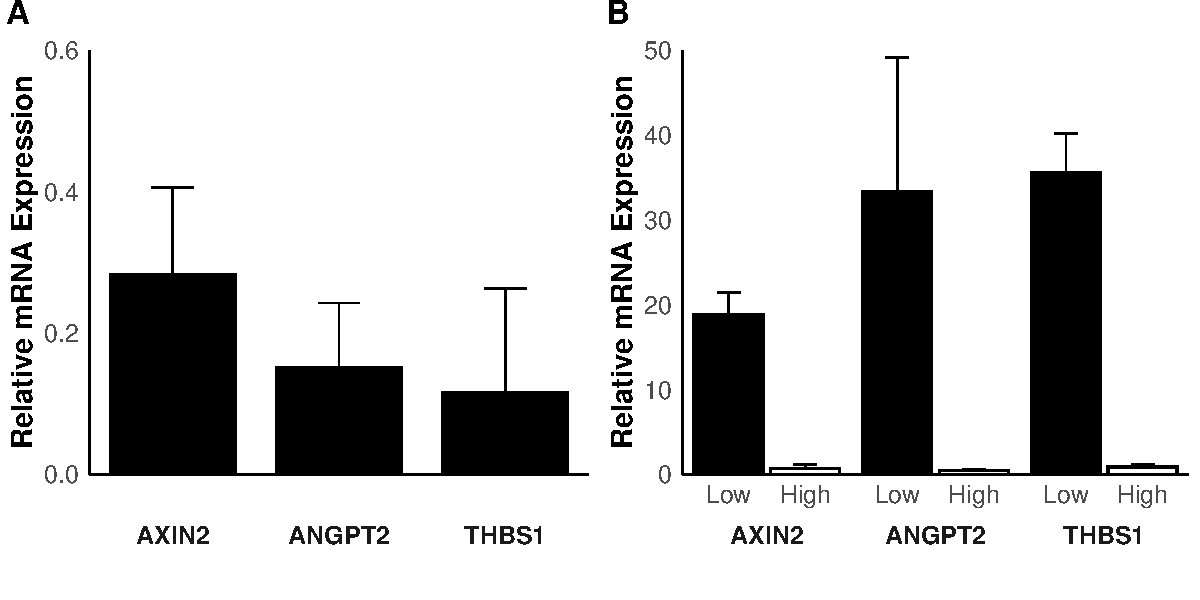
\includegraphics{report_files/figure-latex/plots-1.pdf}
\caption{\label{fig:plots}(\textbf{ABC}) Cells were treated with DMSO(-) or XAV939(+) and exposured to low or high shear stress. Levels of angiopoeitin-2 , axin-2, and thrombospondin-1 mRNA quantified by qPCR. Data is shown as fold change ± SEM, normalised to the HPRT control and relative to the static control. \(^{**}\)\emph{P} \textless{} 0.01, and \(^*\)\emph{P} \textless{} 0.05. (\textbf{DEF}) Under the same conditions, gene expression of cells exposed to low stress are compared to cells exposed to high stress. Data is shown as fold change ± SEM, normalised to the HPRT control and relative to the periphery control. \(^{**}\)\emph{P} \textless{} 0.01, and \(^*\)\emph{P} \textless{} 0.05.}
\end{figure}

\hypertarget{discussion}{%
\section{Discussion}\label{discussion}}

\hypertarget{atheroprotective-gene-expression}{%
\subsection{Atheroprotective gene expression}\label{atheroprotective-gene-expression}}

Limitations of orbital shaker = imporve method

\hypertarget{future}{%
\subsection{Future}\label{future}}

primer specificity test

epigenetics

look at proliferation, apoptosis, senescence, inflammation = PERP, p53

look at vascular repair = wound scratch assay?

look at emt = slug/snail?

\hypertarget{acknowledgements}{%
\section{Acknowledgements}\label{acknowledgements}}

\begin{flushright}
(482 Words) remove headers !!!
\end{flushright}

\hypertarget{references}{%
\section{References}\label{references}}

\hypertarget{refs}{}
\begin{CSLReferences}{0}{0}
\leavevmode\vadjust pre{\hypertarget{ref-howe2020}{}}%
Howe, K. L. {et al.} (2020). {Ensembl 2021}. \emph{Nucleic Acids Research}, 49 (D1), pp.D884--D891. {[}Online{]}. Available at: doi:\href{https://doi.org/10.1093/nar/gkaa942}{10.1093/nar/gkaa942}.

\leavevmode\vadjust pre{\hypertarget{ref-R}{}}%
R Core Team. (2018). {\emph{R: A language and environment for statistical computing}}. Vienna, Austria: R Foundation for Statistical Computing. {[}Online{]}. Available at: \url{https://www.R-project.org/}.

\leavevmode\vadjust pre{\hypertarget{ref-Warboys2019}{}}%
Warboys, C. M., Ghim, M. and Weinberg, P. D. (2019). {Understanding mechanobiology in cultured endothelium: A review of the orbital shaker method}. \emph{Atherosclerosis}, 285, pp.170--177. {[}Online{]}. Available at: doi:\href{https://doi.org/10.1016/j.atherosclerosis.2019.04.210}{10.1016/j.atherosclerosis.2019.04.210}.

\leavevmode\vadjust pre{\hypertarget{ref-Zhu2017}{}}%
Zhu, J. {et al.} (2017). {Regulation of angiogenic behaviors by oxytocin receptor through Gli1-indcued transcription of HIF-1? in human umbilical vein endothelial cells}. \emph{Biomedicine \& Pharmacotherapy}, 90, pp.928--934. {[}Online{]}. Available at: doi:\href{https://doi.org/10.1016/j.biopha.2017.04.021}{10.1016/j.biopha.2017.04.021}.

\end{CSLReferences}

\end{document}
